\documentclass[11pt,a4paper]{article}

\usepackage[margin=2.5cm]{geometry}
\usepackage{amsmath,amssymb}
\usepackage{graphicx}
\usepackage{booktabs}
\usepackage[round,authoryear]{natbib}
\usepackage[colorlinks=true,linkcolor=blue!50!black,citecolor=blue!50!black,urlcolor=blue!50!black]{hyperref}
\usepackage{xcolor}

\graphicspath{{../../figures/}}

\newcommand{\Msun}{M_\odot}
\newcommand{\dd}{\mathrm{d}}
\newcommand{\cl}{\mathrm{cl}}

\title{Compact baryonic clumps as dark matter:\\
what the cosmic microwave background and small-scale structure can tell us}
\author{S\textperiodcentered HARDY\textperiodcentered HOC\textperiodcentered PER\textperiodcentered CLAVDIVM\textperiodcentered FIERI\textperiodcentered IVSSIT}
\date{Draft of 26 September 2026}

\begin{document}
\maketitle

\begin{abstract}
This note explains, from first principles, the physics behind a set of numerical experiments that ask whether some or all of the cosmological dark matter could be made of compact, optically thick clumps of ordinary baryonic matter. The central idea is that the cosmic microwave background (CMB) responds to how matter moves and interacts, while remaining blind to its composition, so a population of clumps that exchanges momentum with radiation only weakly can masquerade as cold dark matter. We describe the linear theory of cosmological perturbations and the photon Boltzmann hierarchy, explain how the public Boltzmann code \textsc{class} models a dark matter component coupled to photons, and summarise what has been found so far. At fixed cosmology the CMB anisotropies become sensitive to a clump population whose momentum-transfer cross-section per unit mass exceeds roughly $4\times10^{-8}\,\mathrm{cm^2\,g^{-1}}$ in an idealised cosmic-variance-limited survey, and the published Planck analysis corresponds to a minimum clump surface density of about $10^6\,\mathrm{g\,cm^{-2}}$. The observable signal arises almost entirely from radiation dragging the clumps at early times, while the photons themselves scatter off the clumps only rarely, and this makes the result insensitive to the detailed angular law of the photon--clump interaction. The same drag suppresses small-scale structure, and matching this suppression to modern warm dark matter limits raises the minimum surface density to about $5\times10^{10}\,\mathrm{g\,cm^{-2}}$. These results are conditional on the clumps existing at the epochs concerned. An order-of-magnitude thermal argument, which sits alongside Big Bang nucleosynthesis as a question about that premise, indicates that clumps held at the radiation temperature remain gravitationally bound only if they are sufficiently massive or dense, and so constrains the clump mass and density that the CMB itself does not probe.
\end{abstract}

\tableofcontents

\section{Motivation and the question being asked}
\label{sec:motivation}

The evidence for dark matter is gravitational: galaxy rotation curves, cluster dynamics, gravitational lensing, and above all the pattern of acoustic peaks in the CMB and the growth of large-scale structure all require a component of matter that does not interact appreciably with light. In the standard cosmological model, $\Lambda$CDM, this component is a new, collisionless, non-baryonic particle, and its density is about five times that of ordinary baryons \citep{Planck2018}. Baryonic candidates for the dark matter are usually dismissed on two grounds. The first is Big Bang nucleosynthesis, which fixes the baryon density at the time light elements formed. The second is the CMB itself, whose acoustic peak heights measure the baryon density at recombination through the inertia that baryons add to the photon--baryon fluid.

The second argument contains an assumption that deserves scrutiny. The CMB measures the density of matter that is \emph{coupled to the photons}, because that is the matter which participates in the acoustic oscillations. Diffuse baryons are tightly coupled to the photons through Thomson scattering off free electrons, but baryons locked into compact, dense objects are not: a clump of mass $M$ and radius $R$ presents a cross-section of order $\pi R^2$ to the radiation, and its cross-section per unit mass $\pi R^2/M$ can be made arbitrarily small by making the clump denser. In the limit of very small cross-section per unit mass, a population of clumps behaves dynamically exactly like cold dark matter. Proposals that the dark matter of galaxies might consist of cold, dense gas clouds have been made on quite different grounds, for example to explain the extreme scattering events seen in radio observations of quasars \citep{WalkerWardle1998}.

The project therefore sets aside, for the moment, the questions of nucleosynthesis and cloud formation, and asks a narrower question that can be answered with standard tools:
\begin{quote}
\emph{If a fraction $f_\cl$ of the dark matter were in compact, pressureless clumps that exchange momentum with photons through an effective cross-section $\sigma$, how large can the cross-section per unit mass $\sigma/M$ be before the CMB, or other probes of structure, notice?}
\end{quote}
For optically thick clumps the cross-section is set by geometry, so a bound on $\sigma/M$ becomes a lower bound on the clump surface density $\Sigma = M/\pi R^2$. The rest of this note builds up the physics needed to answer the question, describes how the numerical calculations are done, and reports the results so far. Sections~\ref{sec:background} and~\ref{sec:perturbations} review standard material and may be skipped by readers familiar with CMB physics; Section~\ref{sec:idm} introduces the photon--clump interaction, Section~\ref{sec:class} explains what the \textsc{class} code computes, and Sections~\ref{sec:results}--\ref{sec:survival} present the results.

\section{The homogeneous universe}
\label{sec:background}

On large scales the universe is described by the Friedmann--Lema\^itre--Robertson--Walker metric, which for a spatially flat universe can be written in terms of conformal time $\tau$ as
\begin{equation}
\dd s^2 = a^2(\tau)\left[-\dd\tau^2 + \delta_{ij}\,\dd x^i \dd x^j\right],
\end{equation}
where $a$ is the scale factor, normalised to unity today, and we use units with $c=1$ in this section. Conformal time is related to cosmic time by $\dd t = a\,\dd\tau$, and a light ray travels a comoving distance $\dd x = \dd\tau$, so $\tau$ is also the comoving size of the causal horizon. The redshift of light emitted at scale factor $a$ is $1+z = 1/a$. The expansion rate $H = \dot a/a$ (a dot denoting $\dd/\dd t$) obeys the Friedmann equation
\begin{equation}
H^2 = \frac{8\pi G}{3}\sum_i \rho_i ,
\end{equation}
where the sum runs over photons, neutrinos, baryons, dark matter and dark energy. It is convenient to use the conformal Hubble rate $\mathcal{H} = a'/a = aH$, where a prime denotes $\dd/\dd\tau$. Cosmologists quote densities through the dimensionless combinations $\omega_i = \Omega_i h^2$, where $\Omega_i$ is the present density in units of the critical density $3H_0^2/8\pi G$ and $H_0 = 100\,h\,\mathrm{km\,s^{-1}\,Mpc^{-1}}$. The project uses a Planck-like reference cosmology with $\omega_b = 0.02237$, $\omega_{\rm dm} = 0.1200$ and $h \approx 0.674$ \citep{Planck2018}.

Matter density scales as $a^{-3}$ and radiation density as $a^{-4}$, so the universe was radiation dominated before matter--radiation equality at $z_{\rm eq}\approx 3400$ and matter dominated afterwards. At early times the photons and baryons form a hot plasma; as the universe cools, electrons and protons combine into neutral hydrogen, the free electron fraction $x_e$ drops rapidly around $z\approx 1100$, and the universe becomes transparent. This epoch is called recombination, and the CMB photons we observe last scattered at that time.

\section{Linear perturbations and the photon Boltzmann hierarchy}
\label{sec:perturbations}

\subsection{Fluid variables}

Structure grows from small initial fluctuations, and while these are small they can be treated with linear perturbation theory. Each Fourier mode of comoving wavenumber $k$ evolves independently. For each species one defines a density contrast $\delta = \delta\rho/\rho$ and a velocity divergence $\theta = ik^j v_j$, and for relativistic species also an anisotropic stress $\sigma$. The metric perturbations require a choice of gauge; \textsc{class} by default uses the synchronous gauge, in which the metric perturbations are described by two scalars $h$ and $\eta$ and in which cold dark matter defines the coordinate system, so that its velocity vanishes identically. The equations used here follow the standard treatment of \citet{MaBertschinger1995}, and a gentler introduction is given in the textbook by \citet{DodelsonSchmidt2020}.

A pressureless, collisionless fluid obeys the continuity and Euler equations
\begin{align}
\delta' &= -\theta - \tfrac12 h', \label{eq:cont}\\
\theta' &= -\mathcal{H}\theta, \label{eq:euler}
\end{align}
so that in the synchronous gauge its velocity, once zero, stays zero, while its density contrast grows under gravity. Baryons obey similar equations with a small pressure term and a coupling to photons that we describe below.

\subsection{The photon distribution function}

Photons cannot be described by a fluid alone, because after recombination they stream freely and their angular distribution matters. One writes the photon temperature at position $\mathbf{x}$, travelling in direction $\hat{\mathbf n}$, as $T(1+\Theta)$, and expands the Fourier-space perturbation in Legendre polynomials of $\mu = \hat{\mathbf k}\cdot\hat{\mathbf n}$,
\begin{equation}
\Theta(k,\mu,\tau) = \sum_{\ell} (-i)^\ell (2\ell+1)\,\Theta_\ell(k,\tau)\,P_\ell(\mu).
\end{equation}
The monopole $\Theta_0$ is related to the density contrast by $\delta_\gamma = 4\Theta_0$, the dipole to the velocity by $\theta_\gamma = 3k\Theta_1$, and the quadrupole to the anisotropic stress by $\sigma_\gamma = 2\Theta_2$. Linear polarization is described by a second function $\Theta_P$ with its own multipoles $\Theta_{P\ell}$.

The Boltzmann equation for $\Theta$ has a free-streaming part, which transfers power from each multipole $\ell$ to its neighbours $\ell\pm1$ at a rate of order $k$, a gravitational part, and a collision term describing Thomson scattering off free electrons. Writing $\dot\kappa \equiv a n_e \sigma_T$ for the conformal Thomson scattering rate (the ``opacity''), the collision term for the temperature multipoles is \citep{DodelsonSchmidt2020}
\begin{equation}
\Theta_\ell' \supset -\dot\kappa\left[\Theta_\ell - \delta_{\ell0}\Theta_0 - \delta_{\ell1}\frac{\theta_b}{3k} - \delta_{\ell2}\frac{\Pi}{10}\right],
\qquad \Pi = \Theta_2 + \Theta_{P0} + \Theta_{P2},
\label{eq:collision}
\end{equation}
and for the polarization multipoles
\begin{equation}
\Theta_{P\ell}' \supset -\dot\kappa\left[\Theta_{P\ell} - \frac{\Pi}{2}\left(\delta_{\ell0} + \frac{\delta_{\ell2}}{5}\right)\right].
\label{eq:collisionP}
\end{equation}
Each term has a transparent physical meaning. Scattering drives every multipole towards zero at the rate $\dot\kappa$, because it randomises photon directions, except that the monopole is conserved (scattering conserves photon number and, to first order, energy) and the dipole is driven towards the bulk velocity of the scatterers. The $\Pi$ terms reflect the angular dependence of Thomson scattering, whose cross-section varies as $1+\cos^2\vartheta$ with the scattering angle: scattering partly regenerates a quadrupole, and a quadrupole anisotropy in the radiation incident on an electron produces linearly polarized scattered light. These $\Pi$ terms are the only place where polarization is generated at linear order, and they will matter in Section~\ref{sec:kernel}.

\subsection{Tight coupling, acoustic oscillations and diffusion damping}

Before recombination the Thomson rate greatly exceeds both the expansion rate and the rate $k$ at which free streaming acts on the modes of interest, so the photons and baryons are locked together into a single fluid. In this tight-coupling limit all multipoles with $\ell\ge2$ are suppressed by powers of $k/\dot\kappa$ and the fluid obeys an oscillator equation, whose solution is an acoustic wave with sound speed
\begin{equation}
c_s = \frac{1}{\sqrt{3(1+R_b)}}, \qquad R_b = \frac{3\rho_b}{4\rho_\gamma},
\end{equation}
where $R_b$ measures the inertia that the baryons add to the fluid. The comoving distance a sound wave can travel before recombination, the sound horizon $r_s = \int c_s\,\dd\tau$, sets the characteristic angular scale of the CMB peaks, and the baryon loading $R_b$ shifts the zero point of the oscillation so that compressional peaks are enhanced relative to rarefaction peaks \citep{HuSugiyama1995}. This is why the CMB measures the baryon density: extra matter that shares the photons' motion changes $R_b$, the sound horizon and the relative heights of odd and even peaks.

The coupling is not perfect. Photons random-walk through the plasma with a mean free path $1/\dot\kappa$, and fluctuations on scales smaller than the distance a photon diffuses in a Hubble time are erased \citep{Silk1968}. The corresponding damping wavenumber is
\begin{equation}
k_D^{-2} = \int \frac{\dd\tau}{6(1+R_b)\dot\kappa}\left[\frac{R_b^2}{1+R_b} + \frac{16}{15}\right],
\end{equation}
and it produces the exponential fall-off of the CMB spectrum at high multipoles, known as the damping tail.

\subsection{From perturbations to observed spectra}

The anisotropy observed today in direction $\hat{\mathbf n}$ is expanded in spherical harmonics, and the statistics of the coefficients are summarised by the angular power spectrum $C_\ell$. In practice one plots $D_\ell = \ell(\ell+1)C_\ell/2\pi$. The efficient way to compute $C_\ell$ is the line-of-sight integral \citep{SeljakZaldarriaga1996},
\begin{equation}
\Theta_\ell(k,\tau_0) = \int_0^{\tau_0} \dd\tau\; S(k,\tau)\, j_\ell\!\left[k(\tau_0-\tau)\right],
\qquad
C_\ell = 4\pi\int \frac{\dd k}{k}\,\mathcal{P}_\mathcal{R}(k)\,\left|\Theta_\ell(k,\tau_0)\right|^2,
\label{eq:los}
\end{equation}
where $j_\ell$ is a spherical Bessel function, $\mathcal{P}_\mathcal{R}$ is the primordial power spectrum, and the source function $S$ contains the physics of the last scattering surface weighted by the visibility function
\begin{equation}
g(\tau) = \dot\kappa\, e^{-\kappa(\tau)},\qquad \kappa(\tau) = \int_\tau^{\tau_0}\dot\kappa\,\dd\tau',
\end{equation}
which is the probability density that a photon observed today last scattered at time $\tau$. The visibility function is sharply peaked at recombination, with a second smaller bump at reionization ($z\approx 8$), which produces the large-angle polarization signal. The source function includes the intrinsic temperature and gravitational potential at last scattering (the Sachs--Wolfe term), the Doppler shift from the scatterers' velocity, the integrated Sachs--Wolfe effect from time-varying potentials, and the polarization term proportional to $g\,\Pi$.

Three spectra are measured with high precision: the temperature spectrum TT, the E-mode polarization spectrum EE, and their cross-correlation TE. A fourth, the lensing potential spectrum $C_L^{\phi\phi}$, describes how the gravitational potential of intervening structure deflects the CMB photons; lensing smooths the acoustic peaks slightly and is sensitive to the matter distribution on scales of a few to tens of megaparsecs \citep{LewisChallinor2006}. The same linear calculation also gives the matter power spectrum $P(k)$, which describes the clustering of matter today.

Even a perfect, full-sky measurement cannot determine $C_\ell$ exactly, because only $2\ell+1$ independent modes exist at each multipole. This cosmic variance sets the fractional uncertainty $\sqrt{2/(2\ell+1)}$, and it is used below to build an idealised measure of detectability,
\begin{equation}
\Delta\chi^2_{\rm CV} = \sum_\ell \frac{\left(C_\ell^{\rm model}-C_\ell^{\rm ref}\right)^2}{\mathrm{Var}(C_\ell)},\qquad \mathrm{Var}(C_\ell)=\frac{2}{2\ell+1}C_\ell^2,
\label{eq:chi2cv}
\end{equation}
which ignores instrumental noise, sky coverage and the freedom to adjust other cosmological parameters. It therefore overstates how well real data constrain a model, and serves only to indicate where the CMB starts to be sensitive.

\section{Dark matter that interacts with photons}
\label{sec:idm}

\subsection{Equations of motion}

Consider now a pressureless component, which we call the clumps, that scatters photons with a cross-section $\sigma$ per object. The clumps have number density $n_\cl$ and mass $M$, so their mass density is $\rho_\cl = n_\cl M$. By analogy with Thomson scattering one defines the conformal photon--clump interaction rate
\begin{equation}
\dot\mu = a\, n_\cl\, \sigma = a\,\rho_\cl\,\frac{\sigma}{M}.
\label{eq:mudot}
\end{equation}
Photon--clump scattering transfers momentum between the photon fluid and the clumps. Following \citet{Boehm2001} and \citet{Wilkinson2014}, the photon and clump Euler equations acquire drag terms of opposite sign,
\begin{align}
\theta_\gamma' &\supset \dot\kappa\,(\theta_b - \theta_\gamma) + \dot\mu\,(\theta_\cl - \theta_\gamma), \label{eq:photon_euler}\\
\theta_\cl' &= -\mathcal{H}\theta_\cl + S\,\dot\mu\,(\theta_\gamma - \theta_\cl), \qquad S = \frac{4\rho_\gamma}{3\rho_\cl}. \label{eq:clump_euler}
\end{align}
The factor $S$ is required by momentum conservation: the momentum density of the photon fluid is $(\rho_\gamma + p_\gamma)\theta_\gamma = \tfrac43\rho_\gamma\theta_\gamma$, so the change in clump momentum must be weighted by the ratio of inertias. It also expresses an important asymmetry. The photons experience the clumps at the rate $\dot\mu$, while each clump experiences the photons at the rate $S\dot\mu$, which is larger by the ratio of radiation to clump inertia. At early times, when radiation dominates, $S \gg 1$ and the clumps can be dragged by the photons even when the photons scarcely notice the clumps. This asymmetry turns out to be the key to the results of this project.

The photon collision terms for $\ell\ge2$ also change. In the treatment used by \textsc{class} the clumps scatter with the same angular law as Thomson scattering, so the clump contribution enters equations~(\ref{eq:collision}) and (\ref{eq:collisionP}) simply by replacing $\dot\kappa$ with $\dot\kappa + \dot\mu$ everywhere \citep{Wilkinson2014, StadlerBoehm2018}. Whether that is appropriate for a macroscopic object is examined in Section~\ref{sec:kernel}.

\subsection{Interaction strength and its physical meaning}

The literature on dark matter--photon scattering parameterises the interaction through the dimensionless quantity
\begin{equation}
u = \frac{\sigma}{\sigma_T}\left(\frac{M}{100\,\mathrm{GeV}}\right)^{-1},
\end{equation}
which compares the cross-section per unit mass with that of Thomson scattering for a 100\,GeV particle. For a macroscopic object the relevant quantity is simply $\sigma/M$, and evaluating the constants gives
\begin{equation}
u \simeq 268\,\left[\frac{\sigma/M}{\mathrm{cm^2\,g^{-1}}}\right].
\end{equation}
Only the combination $\sigma/M$ enters equations~(\ref{eq:mudot})--(\ref{eq:clump_euler}), so the mass of an individual clump never appears in the linear dynamics.

For an optically thick sphere the momentum-transfer cross-section is geometric, $\sigma = Q\pi R^2$, where $Q$ is an efficiency of order unity that depends on how the surface interacts with light. For a perfect absorber that re-emits isotropically in its own rest frame, or for a specularly reflecting sphere, $Q=1$; for a diffusely (Lambertian) reflecting sphere $Q = 13/9$. The strictly relevant quantity for the drag is the momentum-transfer cross-section $\sigma_{\rm mt} = \int (1-\cos\vartheta)\,\dd\sigma$, which for Thomson scattering equals $\sigma_T$ because the scattering is symmetric between forward and backward directions. Writing the clump surface density as $\Sigma = M/\pi R^2$,
\begin{equation}
\frac{\sigma}{M} = \frac{Q}{\Sigma}, \qquad u \simeq \frac{268\,Q}{\Sigma/(\mathrm{g\,cm^{-2}})},
\end{equation}
so an upper limit on $u$ is a lower limit on $\Sigma/Q$. For orientation, $u = 10^{-4}$ corresponds to $\Sigma/Q \approx 2.7\times10^6\,\mathrm{g\,cm^{-2}}$, roughly the column density of ten kilometres of rock, while the column through the whole Earth is about $7\times10^9\,\mathrm{g\,cm^{-2}}$.

\subsection{Interaction rates and decoupling}

Two rates, measured against the expansion rate, characterise the interaction. The photon opacity due to clumps, expressed as a physical rate, is $\Gamma_{\gamma\to\cl} = \dot\mu/a$, and the rate at which the clumps are dragged is $\Gamma_{\cl\to\gamma} = S\,\Gamma_{\gamma\to\cl}$. Because $n_\cl\propto a^{-3}$ and $\rho_\gamma/\rho_\cl\propto a^{-1}$, both ratios $\Gamma/H$ fall with time, and each crosses unity at a characteristic decoupling redshift. The drag rate is the one that controls when the clumps begin to move independently of the radiation, and the redshift $z_{\rm dec}$ at which $\Gamma_{\cl\to\gamma} = H$ is the natural physical summary of the interaction strength.

\subsection{Collisional damping of the matter perturbations}

While the clumps are dragged by the radiation they cannot fall freely into gravitational potential wells; instead they share the oscillating, diffusion-damped motion of the photon fluid. Perturbations on scales that enter the causal horizon while the drag is still effective are therefore damped, much as fluctuations in a free-streaming warm dark matter component are erased on scales below its free-streaming length \citep{Boehm2001}. The result is a cutoff in the matter power spectrum at a wavenumber roughly equal to the horizon scale at $z_{\rm dec}$, below which structure is strongly suppressed. The cutoff is conveniently described by the transfer function $T^2(k) = P(k)/P_{\Lambda\rm CDM}(k)$ and by the half-mode wavenumber $k_{\rm hm}$ at which $T = 1/2$, with the corresponding half-mode mass
\begin{equation}
M_{\rm hm} = \frac{4\pi}{3}\,\bar\rho_m\left(\frac{\lambda_{\rm hm}}{2}\right)^3, \qquad \lambda_{\rm hm} = \frac{2\pi}{k_{\rm hm}},
\end{equation}
which approximately marks the halo mass below which the abundance of dark matter haloes is suppressed \citep{Schneider2012}.

\section{What the CLASS code computes}
\label{sec:class}

\textsc{class} (the Cosmic Linear Anisotropy Solving System) is a public Boltzmann code that solves the equations above for a user-specified cosmology \citep{Lesgourgues2011, Blas2011}. It is organised as a chain of modules. The \emph{background} module integrates the Friedmann equation and tabulates $a(\tau)$, $H$ and all densities. The \emph{thermodynamics} module solves for the recombination history $x_e(z)$, the Thomson opacity $\dot\kappa$, the visibility function, and, when an interacting dark matter species is present, the clump opacity $\dot\mu$. The \emph{perturbations} module integrates the coupled Einstein--Boltzmann system for every Fourier mode from deep in the radiation era to the present, storing the source functions of equation~(\ref{eq:los}). The \emph{transfer} and \emph{harmonic} modules perform the line-of-sight integrals and the integral over the primordial spectrum to produce $C_\ell$, the \emph{lensing} module applies the lensing deflection to the CMB spectra, and $P(k)$ is extracted along the way.

Since version~3.2, \textsc{class} includes a general interacting dark matter species, called \texttt{idm}, which can scatter with photons, baryons or a dark radiation component \citep{Becker2021}. Its photon coupling implements the formalism of \citet{StadlerBoehm2018}, with the interaction strength set by the parameter \texttt{u\_idm\_g}, the dark matter mass by \texttt{m\_idm}, and an optional temperature dependence of the cross-section through \texttt{n\_index\_idm\_g}. In this project the clumps are represented by the \texttt{idm} species with density \texttt{omega\_idm} $= f_\cl\,\omega_{\rm dm}$, a cross-section independent of temperature (\texttt{n\_index\_idm\_g = 0}), and a very large particle mass.

The particle mass matters only through the thermal velocity of the dark matter, which \textsc{class} includes as a sound speed $c^2_{\rm idm} \propto T_{\rm idm}/m_{\rm idm}$. A macroscopic clump has no appreciable thermal velocity, so the mass must be chosen large enough that this term is negligible. We found that the outputs stop depending on the mass above about $10^{7}$--$10^{8}\,\mathrm{eV}$ and become identical to machine precision above $10^{24}\,\mathrm{eV}$, and all calculations use $m_{\rm idm} = 10^{27}\,\mathrm{eV}$, so that the clump mass drops out exactly, as it should.

Obtaining reliable results at the level of $10^{-4}$ required some care, and the lessons are recorded in the project's implementation notes. The default precision of \textsc{class} is designed for an accuracy of about $10^{-3}$ in a single model, and comparisons between closely related models revealed three numerical effects that are larger than the tolerance. The thermodynamics table had to be sampled four times more finely than the default, because the code moves the start of that table when an interacting species is present, and the resulting change in sampling alone altered the EE spectrum by $2\times10^{-3}$. The perturbation integration had to start ten times earlier than the default, because the code initialises the \texttt{idm} velocity equal to the photon velocity, which is correct only for a tightly coupled species and seeds a small spurious velocity when the coupling is weak. Finally, the spacing of the multipoles at which $C_\ell$ is evaluated had to be halved, because with the default spacing about a third of the models acquired a deterministic error of about $10^{-3}$ at particular sampled multipoles, switching on and off unpredictably as the coupling was varied. With these settings, a model in which all the dark matter is replaced by non-interacting \texttt{idm} reproduces standard $\Lambda$CDM to better than $4\times10^{-5}$ in every spectrum (Figure~\ref{fig:m2a}).

\begin{figure}
\centering
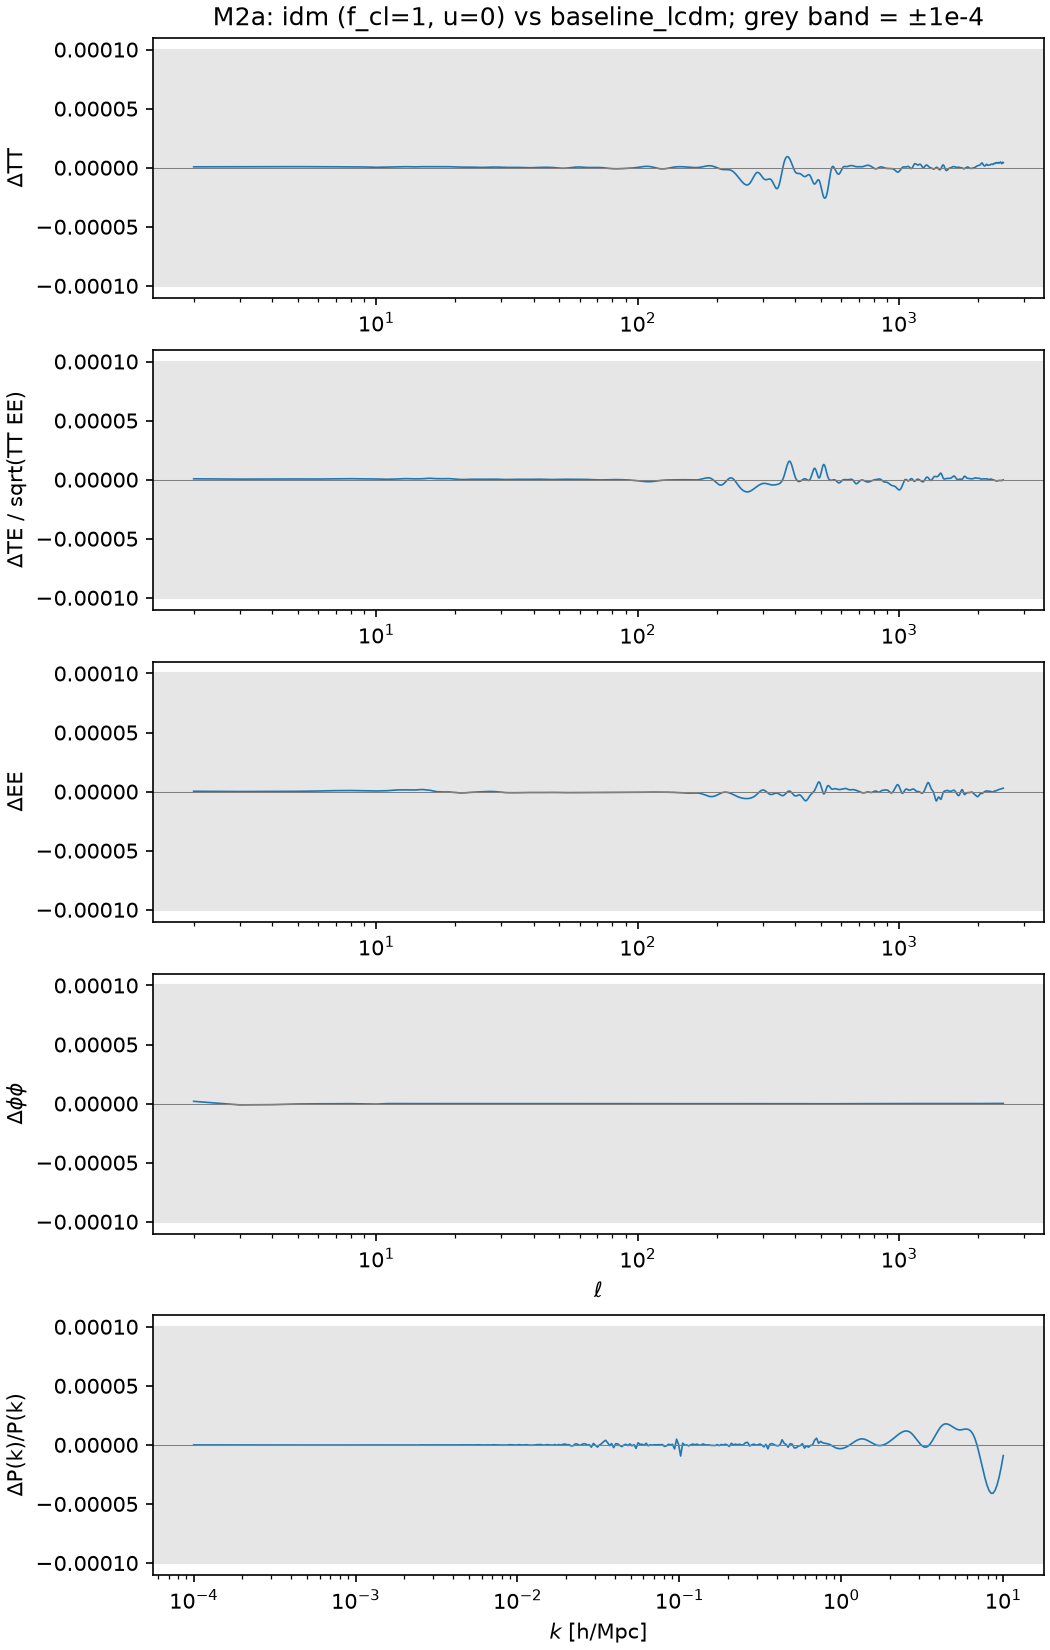
\includegraphics[width=0.62\textwidth]{m2a_residuals.png}
\caption{Validation of the method. Fractional differences between a model in which all the dark matter is the \texttt{idm} species with zero coupling and the reference $\Lambda$CDM model, for (top to bottom) TT, TE, EE, the lensing potential and the matter power spectrum. The grey band shows the $10^{-4}$ tolerance.}
\label{fig:m2a}
\end{figure}

\section{How the CMB responds to photon--clump coupling}
\label{sec:results}

\subsection{The coupling scan}

With all the dark matter in clumps ($f_\cl = 1$) and all other cosmological parameters held fixed, the coupling was varied from $u = 10^{-8}$ to $u = 10^{-1}$, the largest value at which the standard code still runs. Figure~\ref{fig:tt} shows the temperature spectrum and its fractional change, and Table~\ref{tab:scan} summarises representative models. For reference, the published analysis of Planck data by \citet{StadlerBoehm2018} excludes $u > 2.25\times10^{-4}$ at 95\% confidence, which corresponds to $\Sigma/Q > 1.2\times10^6\,\mathrm{g\,cm^{-2}}$.

\begin{figure}
\centering
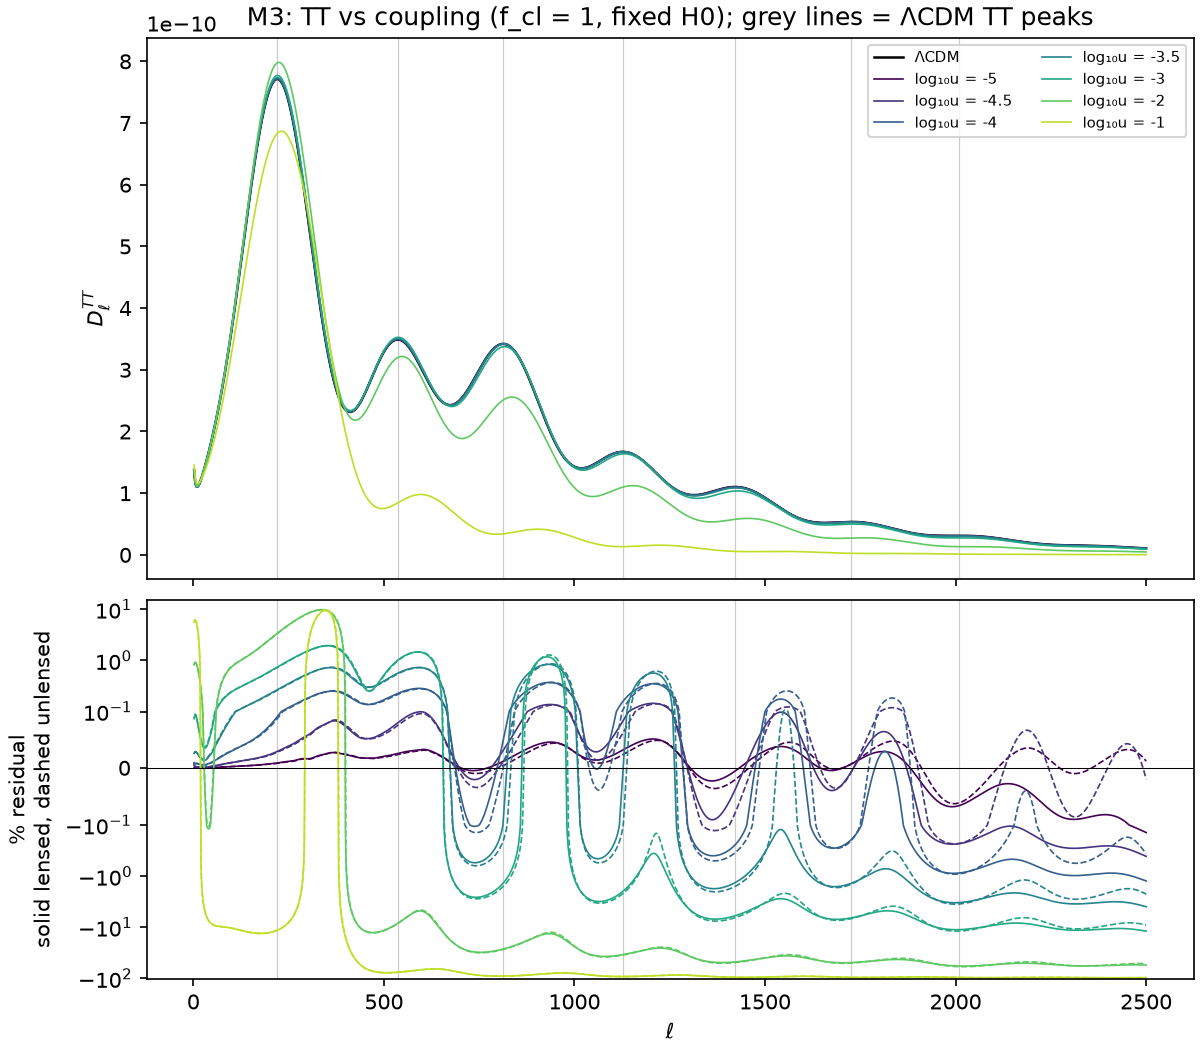
\includegraphics[width=0.85\textwidth]{m3_tt.png}
\caption{Temperature power spectrum for a range of photon--clump couplings with all dark matter in clumps and the other cosmological parameters fixed. The lower panel shows the percentage difference from $\Lambda$CDM (solid lines lensed, dashed lines unlensed); grey vertical lines mark the $\Lambda$CDM acoustic peaks.}
\label{fig:tt}
\end{figure}

\begin{table}
\centering
\caption{Response to the photon--clump coupling at $f_\cl=1$ and fixed cosmology. The maximum fractional changes are taken over $2\le\ell\le2500$ for the lensed spectra; $\Delta\chi^2_{\rm CV}$ is the idealised cosmic-variance statistic of equation~(\ref{eq:chi2cv}) for TT alone; $z_{\rm dec}$ is the redshift at which the clump drag rate equals the expansion rate.}
\label{tab:scan}
\small
\setlength{\tabcolsep}{4pt}
\begin{tabular}{lccccccc}
\toprule
$u$ & $\Sigma/Q$ [g\,cm$^{-2}$] & $z_{\rm dec}$ & max $\Delta C^{TT}_\ell$ & max $\Delta C^{\phi\phi}_L$ & $\Delta\chi^2_{\rm CV}$ (TT) & $\sigma_8$ & $k_{\rm hm}$ [$h$\,Mpc$^{-1}$] \\
\midrule
$0$ ($\Lambda$CDM) & -- & -- & -- & -- & -- & 0.811 & -- \\
$1.1\times10^{-5}$ & $2.4\times10^7$ & $1.7\times10^5$ & 0.15\% & 13\% & 1 & 0.805 & 2.0 \\
$10^{-4}$ & $2.7\times10^6$ & $5.6\times10^4$ & 1.2\% & 54\% & 94 & 0.770 & 0.72 \\
$2.25\times10^{-4}$ & $1.2\times10^6$ & $3.8\times10^4$ & 2.8\% & 75\% & 608 & 0.733 & 0.50 \\
$10^{-3}$ & $2.7\times10^5$ & $1.8\times10^4$ & 12\% & 97\% & $1.7\times10^4$ & 0.606 & 0.27 \\
\bottomrule
\end{tabular}
\end{table}

Several features of the response stand out. The largest and earliest changes in the temperature spectrum appear in the damping tail, where power is removed, while the first few peaks are slightly enhanced. The peaks also move to slightly higher multipoles, by roughly one multipole at $u=10^{-4}$. The lensing potential is by far the most sensitive observable: it changes by one per cent already at $u\approx6\times10^{-7}$, because it responds directly to the suppression of matter clustering on intermediate scales. Lensing roughly doubles the change in the lensed temperature spectrum at small couplings. The idealised statistic of equation~(\ref{eq:chi2cv}) reaches unity at $u\approx1.1\times10^{-5}$ in each of TT, TE and EE; that this is about twenty times below the published Planck bound is expected, since real data have noise, cover part of the sky, and allow the other parameters to adjust.

\subsection{Why the photons hardly notice the clumps}

The rates computed by \textsc{class} (Figure~\ref{fig:rates}) explain these results. At the Planck bound the photon opacity due to clumps is at most $1.1\times10^{-4}$ of the Thomson opacity before recombination, and the total optical depth to clump scattering between recombination and today is only $\tau_\cl\approx10^{-3}$, compared with $0.054$ for reionization. At recombination itself $\Gamma_{\gamma\to\cl}/H \approx 1.5\times10^{-3}$, so a CMB photon has roughly a one in a thousand chance of meeting a clump in a Hubble time. The photons, in other words, scarcely see the clumps.

The clumps, however, feel the photons strongly. Because of the factor $S$ in equation~(\ref{eq:clump_euler}), the drag rate exceeds the expansion rate until $z_{\rm dec}\approx 4\times10^{4}$ at the Planck bound, well before recombination. Every mode that enters the horizon before this epoch, which means every wavenumber above about $0.2\,h\,\mathrm{Mpc^{-1}}$, has its clump perturbation suppressed. The CMB then responds to the weaker gravitational potentials that result: acoustic driving is modified, which changes the peak heights and the damping tail, and there is less structure to lens the CMB. The signal is thus gravitational in origin, transmitted from the dragged clumps to the photons through the metric, with direct scattering of photons off clumps near last scattering playing only a minor role.

\begin{figure}
\centering
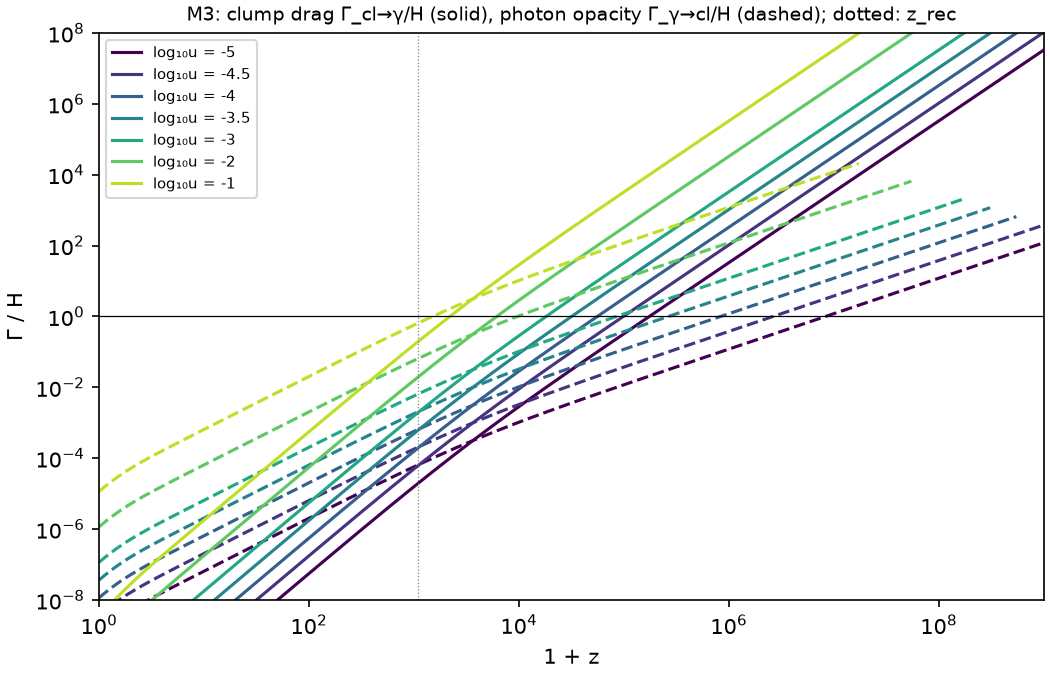
\includegraphics[width=0.72\textwidth]{m3_rates.png}
\caption{Interaction rates relative to the expansion rate for several couplings. Solid lines show the clump drag rate $\Gamma_{\cl\to\gamma}/H$ and dashed lines the photon opacity due to clumps $\Gamma_{\gamma\to\cl}/H$; the dotted vertical line marks recombination. The drag rate is larger by the factor $S = 4\rho_\gamma/3\rho_\cl$, which is large in the radiation era.}
\label{fig:rates}
\end{figure}

\subsection{The strong-coupling limit}

If the clumps were perfectly coupled to the photons throughout the acoustic epoch they would add their inertia to the fluid exactly as baryons do, replacing $R_b$ by $3(\rho_b+\rho_\cl)/4\rho_\gamma$. This would shrink the sound horizon to 0.73 of its standard value and shift the acoustic peaks to multipoles about 37\% higher. At the strongest coupling that the standard code can handle, $u=0.1$, the peaks move by between 5\% and 11\%, because even then the drag becomes ineffective at $z\approx2200$, shortly before recombination. The approach to the photon-loaded limit is therefore partial, and stronger couplings would require modifications to the code, which fails first because its initial conditions assume a tight-coupling approximation that is already switched off, and then because clump opacity pushes the peak of the visibility function below a hard-coded minimum redshift.

\section{Does the angular law of the interaction matter?}
\label{sec:kernel}

The Thomson form of the collision terms in equations~(\ref{eq:collision}) and (\ref{eq:collisionP}) describes an elementary particle. An optically thick macroscopic object interacts with radiation through a different law. A perfect absorber, for example, removes photons from every direction and re-emits them isotropically in its own rest frame, which generates neither a quadrupole nor polarization. To test whether this matters, the \textsc{class} source was modified so that the clump part of the collision term carries two coefficients, $c_T$ multiplying the regeneration of the temperature quadrupole and $c_E$ multiplying the polarization source. The $\ell=2$ temperature equation and the polarization equations become
\begin{align}
\Theta_2' &\supset -(\dot\kappa+\dot\mu)\,\Theta_2 + (\dot\kappa + c_T\dot\mu)\,\frac{\Pi}{10},\\
\Theta_{P\ell}' &\supset -(\dot\kappa+\dot\mu)\,\Theta_{P\ell} + (\dot\kappa + c_E\dot\mu)\,\frac{\Pi}{2}\left(\delta_{\ell0}+\frac{\delta_{\ell2}}{5}\right),
\end{align}
with the corresponding factors applied to the visibility function in the polarization-dependent parts of the line-of-sight sources. Damping of all multipoles with $\ell\ge2$ is unchanged, and so is the momentum exchange of equations~(\ref{eq:photon_euler}) and (\ref{eq:clump_euler}), which depends on the interaction only through $\sigma_{\rm mt}$. The Thomson case is $c_T = c_E = 1$ and the perfect absorber is $c_T = c_E = 0$. The tight-coupling approximation used by \textsc{class} at early times also contains the Thomson law, and its closure relations were generalised exactly; for example, the photon anisotropic stress in the tight-coupling limit becomes $\sigma_\gamma = \tfrac{4}{15}(\theta_\gamma + \ldots)/D$ with
\begin{equation}
D = (\dot\kappa+\dot\mu) - \frac{0.8\,(\dot\kappa + c_T\dot\mu)}{8 - 4.8\,r}, \qquad r = \frac{\dot\kappa + c_E\dot\mu}{\dot\kappa + \dot\mu},
\end{equation}
which reduces to the familiar $\tfrac{16}{45}(\theta_\gamma+\ldots)/(\dot\kappa+\dot\mu)$ for the Thomson law. With Thomson coefficients the modified code reproduces the standard code bit for bit.

\begin{figure}
\centering
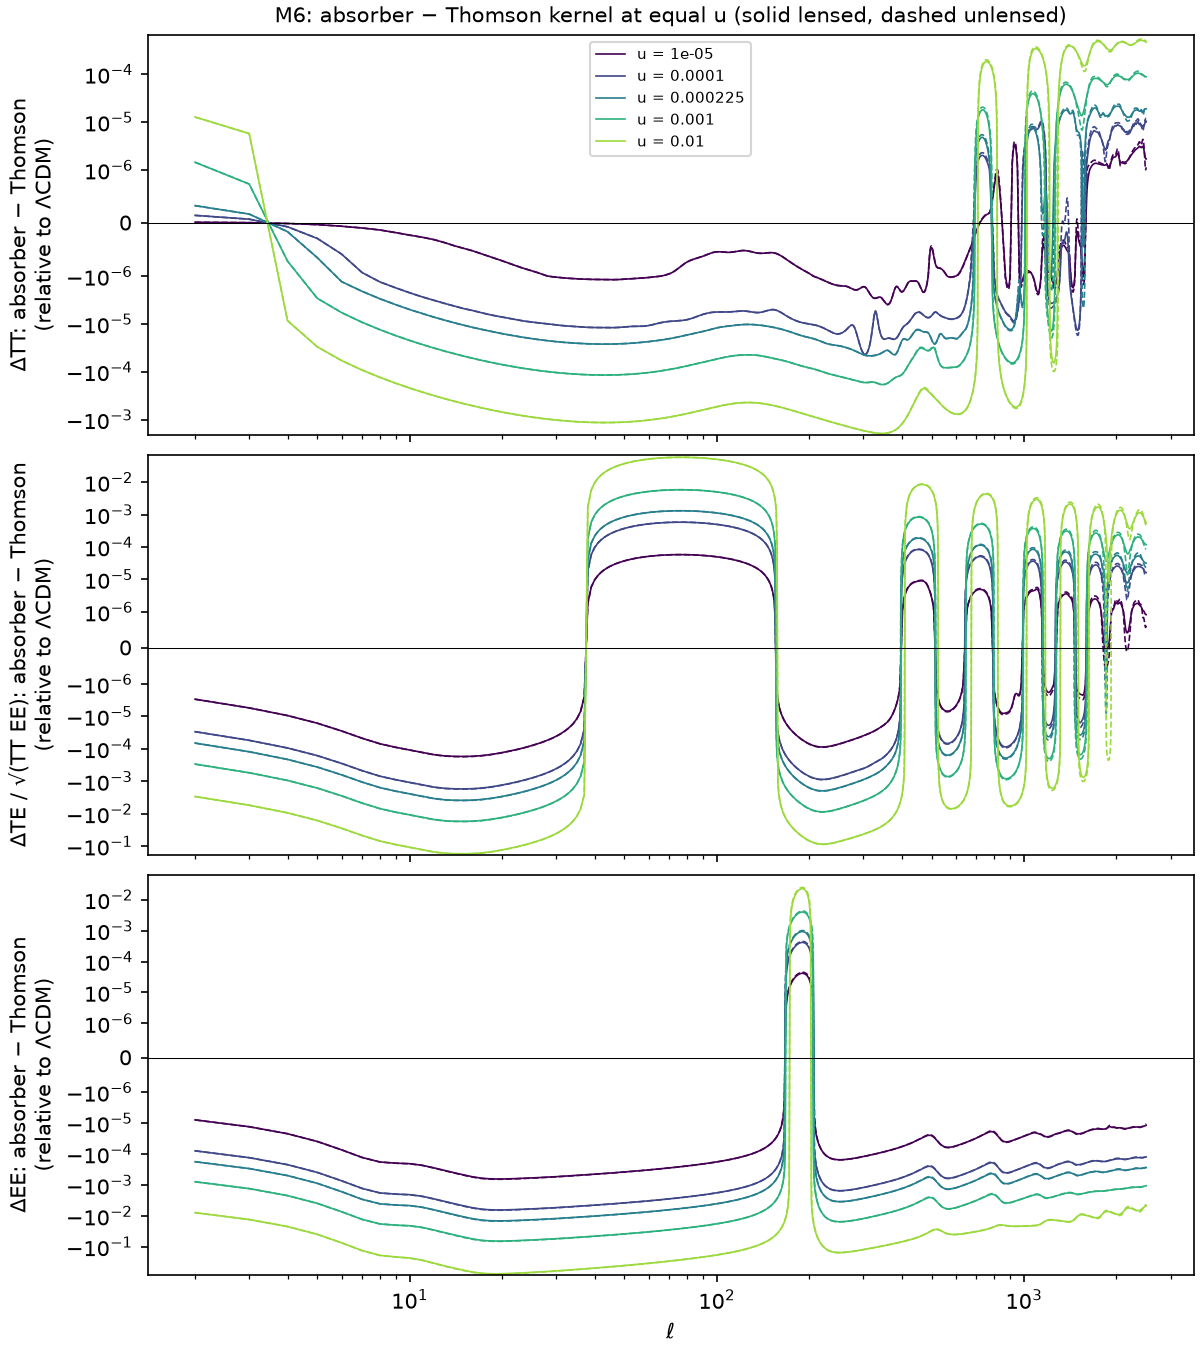
\includegraphics[width=0.75\textwidth]{m6_absorber_vs_thomson.png}
\caption{Difference between a perfect-absorber clump and a Thomson-scattering clump at the same momentum-transfer coupling, relative to $\Lambda$CDM, for TT, TE and EE. Solid lines are lensed and dashed lines unlensed spectra. The temperature spectrum is essentially unchanged, while EE is reduced because an absorber generates no polarization.}
\label{fig:kernel}
\end{figure}

The comparison (Figure~\ref{fig:kernel}) confirms the expectation from the previous section. At equal $u$, the absorber leaves the temperature spectrum, the lensing potential and the matter power spectrum unchanged to within about $5\times10^{-5}$ at the Planck bound. The one genuine difference is in the polarization: clumps that scatter like electrons generate a small amount of polarization, and absorbers do not, so the EE spectrum of the absorber model is lower by up to 1.4\% at the Planck bound, most strongly at $\ell\approx15$--$30$. Setting only $c_E$ to zero reproduces this entire difference, while setting only $c_T$ to zero has an effect several hundred times smaller. Including the correlation of this difference with the main signal, the idealised detectability of the coupling changes by less than one per cent. The conclusion is that the CMB constraint derived for an elementary scatterer applies to opaque clumps, with the interaction law entering only through the efficiency $Q$ in the conversion from $u$ to $\Sigma$.

\section{Small-scale structure}
\label{sec:smallscale}

The drag-induced cutoff in the matter power spectrum (Figure~\ref{fig:pk}) is much more severe than anything the CMB can detect. At the Planck bound the half-mode mass is about $9\times10^{13}\,h^{-1}\Msun$, and $\sigma_8$, the amplitude of matter fluctuations on scales of $8\,h^{-1}$\,Mpc, is reduced by ten per cent; structure below the scale of galaxy clusters would be strongly suppressed. Since galaxies and small satellite galaxies plainly exist, observations of small-scale structure should constrain the coupling far more strongly than the CMB.

\begin{figure}
\centering
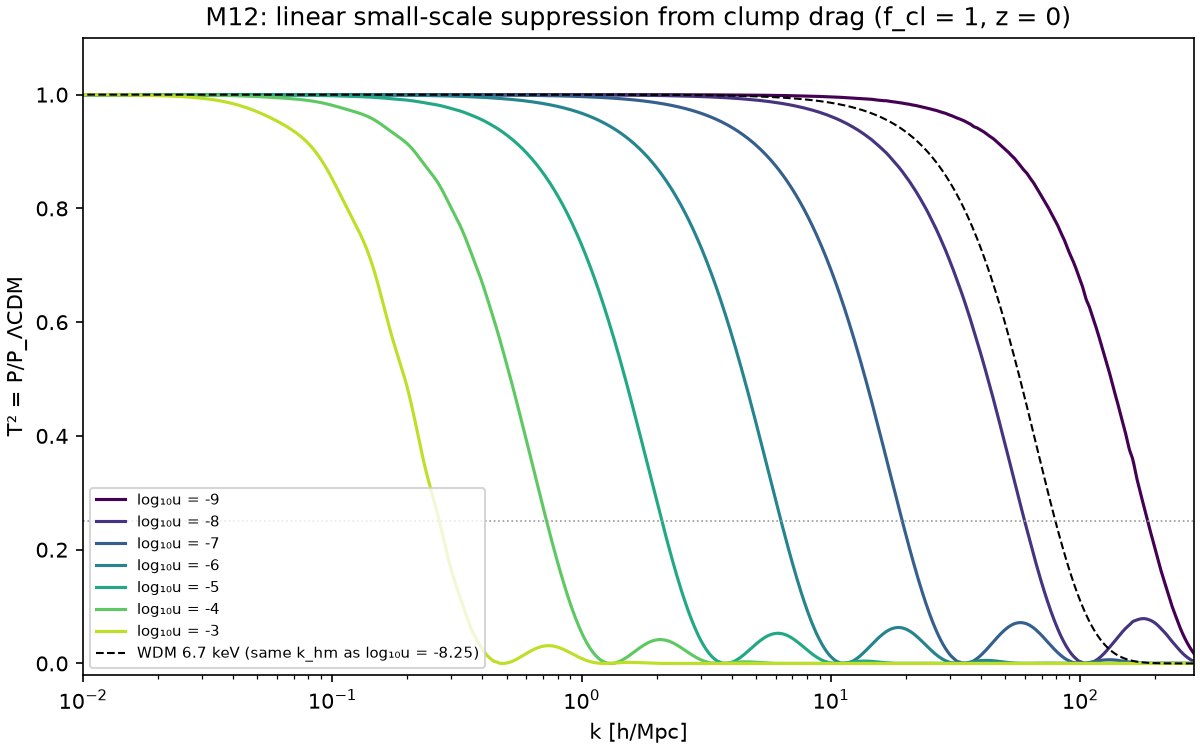
\includegraphics[width=0.72\textwidth]{m12_transfer.png}
\caption{Linear matter transfer function $T^2 = P/P_{\Lambda\rm CDM}$ at $z=0$ for couplings from $u=10^{-9}$ to $10^{-3}$, with all dark matter in clumps. The dashed line is a thermal-relic warm dark matter model with the same half-mode wavenumber as the $u = 10^{-8.25}$ clump model. The clump models show the damped oscillations characteristic of a species that was coupled to an oscillating fluid.}
\label{fig:pk}
\end{figure}

The only direct constraint in the literature on dark matter--photon scattering from small scales comes from N-body simulations of Milky Way-like haloes compared with the observed satellite population, which give $u < 5.5\times10^{-7}$ \citep{Boehm2014}. Much tighter limits exist for thermal-relic warm dark matter, whose transfer function has a similar shape, and we translate them using the half-mode wavenumber. The warm dark matter transfer function is well described by \citep{Viel2005}
\begin{equation}
T_{\rm WDM}(k) = \left[1 + (\alpha k)^{2\nu}\right]^{-5/\nu},\qquad
\alpha = 0.049\left(\frac{m_{\rm WDM}}{\mathrm{keV}}\right)^{-1.11}\left(\frac{\Omega_{\rm WDM}}{0.25}\right)^{0.11}\left(\frac{h}{0.7}\right)^{1.22}h^{-1}\,\mathrm{Mpc},
\end{equation}
with $\nu = 1.12$. A clump model is assigned the warm dark matter mass that has the same $k_{\rm hm}$. The clump half-mode scale follows $k_{\rm hm}\approx 10^{-2.05}\,u^{-0.48}\,h\,\mathrm{Mpc^{-1}}$ over the range studied. The current limits $m_{\rm WDM} > 6.5\,$keV from Milky Way satellites \citep{Nadler2021} and $m_{\rm WDM}>5.3\,$keV from the Lyman-$\alpha$ forest \citep{Irsic2017} then translate into the bounds of Table~\ref{tab:smallscale}.

\begin{table}
\centering
\caption{Upper limits on the coupling $u$ and lower limits on the clump surface density $\Sigma/Q$ for $f_\cl = 1$. Where two values are given, the first uses the fitting formula of \citet{Viel2005} for the warm dark matter half-mode scale and the second uses \textsc{class}'s own thermal-relic warm dark matter calculation, which gives an 11--17\% larger $k_{\rm hm}$ at the relevant masses.}
\label{tab:smallscale}
\begin{tabular}{lcc}
\toprule
Constraint & $u_{\max}$ & $(\Sigma/Q)_{\min}$ [g\,cm$^{-2}$] \\
\midrule
CMB anisotropies \citep{StadlerBoehm2018} & $2.25\times10^{-4}$ & $1.2\times10^6$ \\
Milky Way satellites, direct \citep{Boehm2014} & $5.5\times10^{-7}$ & $4.9\times10^8$ \\
Lyman-$\alpha$, $m_{\rm WDM}>5.3$\,keV (half-mode) & $(7.2$--$9.6)\times10^{-9}$ & $(2.8$--$3.7)\times10^{10}$ \\
Milky Way satellites, $m_{\rm WDM}>6.5$\,keV (half-mode) & $(4.4$--$6.1)\times10^{-9}$ & $(4.4$--$6.1)\times10^{10}$ \\
\bottomrule
\end{tabular}
\end{table}

These bounds are about ten thousand times tighter in $u$ than the CMB bound, and they carry a systematic uncertainty of perhaps a factor of two from the half-mode matching, since the clump transfer function begins to fall slightly earlier than the warm dark matter one but retains more power beyond the half-mode scale. Two further caveats are important. First, the matching assumes that the clumps behave as a smooth fluid on the half-mode scale; the discreteness of the clumps adds Poisson fluctuations that would rival the adiabatic power at that scale only for clump masses of a few solar masses, so planetary-mass clumps are safely in the fluid regime. Second, and more consequentially, the half-mode scales of these limits entered the horizon at $z\approx 1$--$2\times10^{7}$, when the photon temperature was a few keV. The bound applies only if clumps with the required surface density already existed at that epoch.

\section{Energy exchange, spectral distortions and clump survival}
\label{sec:survival}

\subsection{Spectral distortions}

Thomson scattering conserves photon energy to first order, but an opaque clump absorbs photons and re-emits them at its own temperature. In the early universe, energy injected into the photon field at redshifts between about $5\times10^4$ and $2\times10^6$ cannot be fully thermalised and leaves a chemical-potential (or $\mu$-type) distortion of the blackbody spectrum, while energy injected at later times produces a Compton $y$-type distortion. For an energy release $Q(z)$ per unit volume, these are approximately \citep{Chluba2016}
\begin{equation}
\mu \approx 1.401\int \frac{\dd (Q/\rho_\gamma)}{\dd z}\,J_\mu(z)\,\dd z,\qquad
y \approx \frac14\int \frac{\dd (Q/\rho_\gamma)}{\dd z}\,J_y(z)\,\dd z,
\end{equation}
with visibility functions
\begin{equation}
J_\mu = e^{-(z/z_{\rm th})^{5/2}}\left\{1 - \exp\!\left[-\left(\frac{1+z}{5.8\times10^4}\right)^{1.88}\right]\right\},\qquad
J_y = \left[1+\left(\frac{1+z}{6\times10^4}\right)^{2.58}\right]^{-1},
\end{equation}
and $z_{\rm th}\approx1.98\times10^6$. The COBE/FIRAS measurements limit $|\mu|<9\times10^{-5}$ and $|y|<1.5\times10^{-5}$ \citep{Fixsen1996}.

A clump in an isotropic blackbody radiation field at temperature $T_\gamma$ absorbs power $\pi R^2 c\,aT_\gamma^4$ and emits $\pi R^2 c\,aT_\cl^4$, so its surface relaxes towards $T_\gamma$ on the timescale
\begin{equation}
t_{\rm th} = \frac{\Sigma\,c_v}{4c\,aT_\gamma^3},
\end{equation}
where $c_v$ is the specific heat of the clump material and $a$ here denotes the radiation constant. This is shorter than the Hubble time by many orders of magnitude at every relevant epoch, so the clumps are thermally locked to the CMB. A passive clump that simply follows the cooling radiation releases its heat into the photons, and the total energy exchanged is therefore limited by the heat capacity of the clumps, amounting to about $10^{-9}$ of the photon energy per expansion time. The resulting distortions, $\mu\approx2\times10^{-8}$ and $y\approx3\times10^{-9}$, are thousands of times below the FIRAS limits. Spectral distortions constrain only more exotic clump physics: an internal luminosity per unit mass above about $850\,L_\odot/\Msun$, or a sustained temperature difference between clumps and radiation larger than a few parts per million at the CMB-bound coupling.

\subsection{Can the clumps survive?}

Thermal locking has a more striking consequence. A clump held at the radiation temperature is gravitationally bound only if the gravitational binding energy per particle exceeds the thermal energy, $GM\bar m/R \gtrsim kT_\gamma$, where $\bar m = 0.59\,m_p$ is the mean mass per particle of ionised gas. Writing $M = \pi R^2\Sigma$, this requires
\begin{equation}
M \gtrsim M_{\min}(z,\Sigma) = \frac{1}{\pi\Sigma}\left(\frac{kT_\gamma}{G\bar m}\right)^2,
\end{equation}
or equivalently, for a clump of mean internal density $\rho$, it requires the radiation temperature to have fallen below
\begin{equation}
kT_{\max} = \frac{4\pi G\rho\,\bar m}{3}\left(\frac{3M}{4\pi\rho}\right)^{2/3}.
\end{equation}
Figure~\ref{fig:survival} shows $M_{\min}$ for the surface densities of interest. An Earth-mass clump with a density of $1\,\mathrm{g\,cm^{-3}}$ can be bound only below $z\approx450$, after recombination; a Jupiter-mass clump only below $z\approx4.5\times10^4$; and at $z\sim10^7$, where the small-scale bounds apply, a clump with $\Sigma\sim5\times10^{10}\,\mathrm{g\,cm^{-2}}$ must exceed about ten solar masses. Radiative diffusion heats planetary-mass clumps through within a Hubble time at $z\lesssim10^5$--$10^6$, so the argument is not evaded by an isolated heated surface layer at those epochs, although a massive, cold core losing its outer layers by ablation would survive longer than this simple estimate suggests.

\begin{figure}
\centering
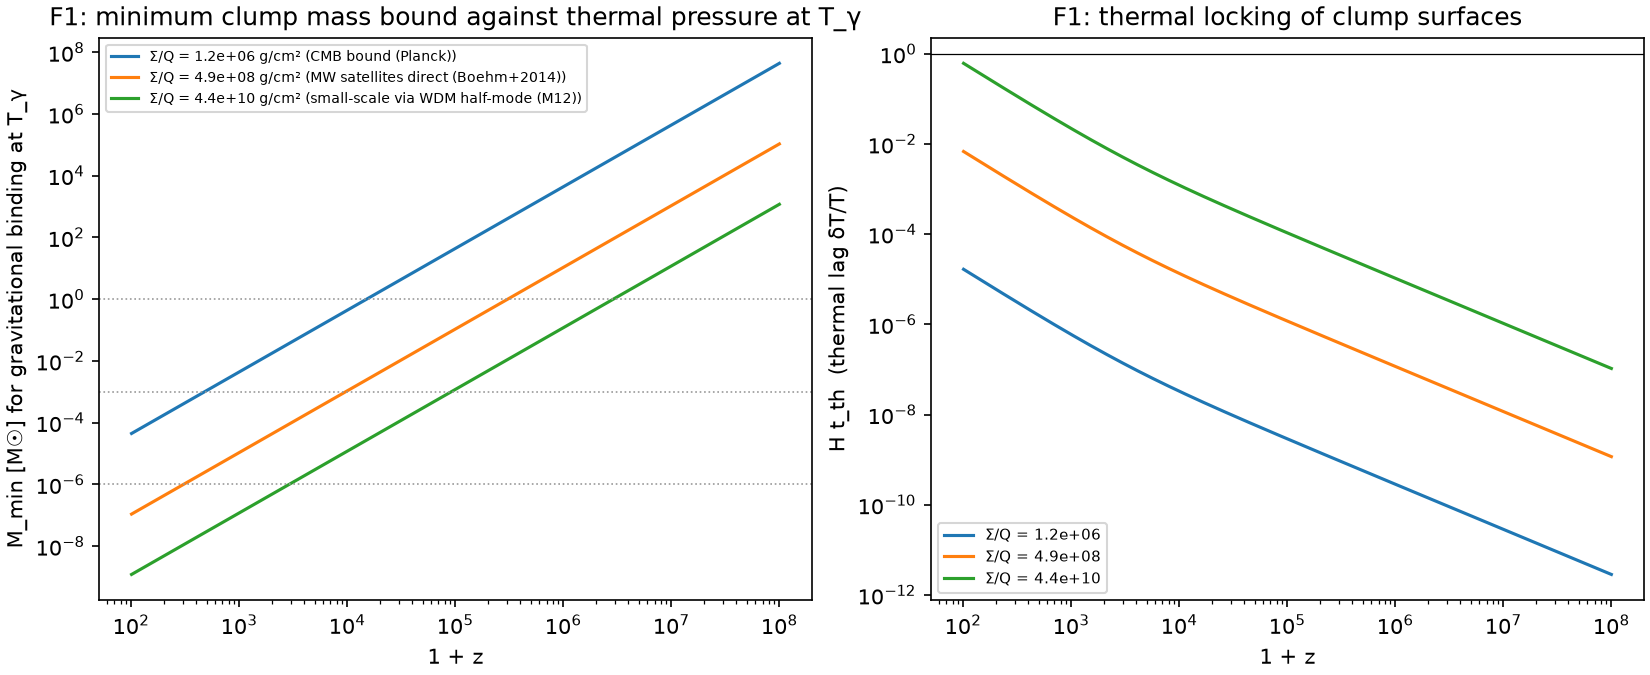
\includegraphics[width=0.95\textwidth]{m13_thermal.png}
\caption{Left: minimum clump mass that remains gravitationally bound when heated to the radiation temperature, for three surface densities corresponding to the CMB, direct satellite and small-scale bounds. Horizontal dotted lines mark $10^{-6}$, $10^{-3}$ and $1\,\Msun$. Right: thermal lag of clump surfaces behind the radiation temperature, which is small at all epochs.}
\label{fig:survival}
\end{figure}

This criterion should be read alongside the constraints of the previous sections, which it complements. The CMB and small-scale bounds limit only the surface density $\Sigma$, because the clump mass drops out of the linear dynamics, whereas the survival criterion limits the mass and internal density at a given epoch. Clumps that satisfy the CMB must be present throughout the acoustic epoch, since extra baryons that were diffuse before recombination would load the photon--baryon fluid, and the small-scale bound assumes their presence as early as $z\sim10^7$. Taken together, the estimates indicate that clumps meeting these conditions would have to be considerably more massive or denser than planetary bodies of ordinary density, and in the most demanding case of stellar mass or of degenerate density. Like the constraint from Big Bang nucleosynthesis, this bears on whether the premise of the calculation can be realised, and it leaves the conditional results of the previous sections unchanged.

\section{Summary and outlook}
\label{sec:summary}

The calculations described here establish four results. The CMB is sensitive to a population of photon-coupled clumps through the drag that radiation exerts on them in the radiation era, which suppresses their clustering and changes the gravitational potentials seen by the photons; the photons themselves barely scatter off the clumps at CMB-relevant couplings. Because the drag depends only on the momentum-transfer cross-section, the constraint derived for an elementary scatterer applies to opaque macroscopic clumps, and the published Planck analysis implies a minimum surface density of about $10^6\,\mathrm{g\,cm^{-2}}$. The same drag produces a cutoff in the matter power spectrum that, when compared with modern warm dark matter limits, raises the minimum surface density to roughly $5\times10^{10}\,\mathrm{g\,cm^{-2}}$, provided the clumps existed by $z\sim10^7$. Finally, spectral distortions provide no useful limit on passive clumps, and a simple thermal argument shows that clumps held at the radiation temperature can remain gravitationally bound only if they are sufficiently massive or dense, a condition on the premise of the calculation that stands beside the familiar constraint from Big Bang nucleosynthesis.

The next stage of the project completes the answer to the conditional question with a proper statistical treatment. A detectability measure that includes instrumental noise and partial sky coverage will be followed by a likelihood analysis against real CMB data, which will first reproduce the published Planck bound as a test of the pipeline, then allow the standard cosmological parameters to adjust, and finally extend the constraint to populations in which only part of the dark matter is clumped. Questions about how and when the clumps could form, together with nucleosynthesis and the survival criterion, will be revisited once that conditional answer is in hand.

All of these results share a second kind of conditionality, distinct from the question of whether the clumps can exist at all. The clumps are the only departure from the standard model in these calculations: recombination is homogeneous, the diffuse baryons form a smooth fluid, there are no magnetic fields and the initial conditions are adiabatic. A population of compact baryonic clumps would have to form from large early inhomogeneities in the baryons, and that process would probably leave other traces, such as small-scale clumping of the remaining gas, which changes the recombination history because recombination depends on the square of the density \citep{JedamzikSaveliev2019}. The limits derived here should therefore be read as statements about a deliberately narrow model, which isolates the effect of the drag, and not as model-independent measurements of the properties of baryonic clumps.

\begin{thebibliography}{99}

\bibitem[Becker et~al.(2021)]{Becker2021}
Becker N., Hooper D.~C., Kahlhoefer F., Lesgourgues J., Sch\"oneberg N., 2021, \emph{Cosmological constraints on multi-interacting dark matter}, JCAP 02, 019.

\bibitem[Blas et~al.(2011)]{Blas2011}
Blas D., Lesgourgues J., Tram T., 2011, \emph{The Cosmic Linear Anisotropy Solving System (CLASS) II: approximation schemes}, JCAP 07, 034.

\bibitem[Boehm et~al.(2001)]{Boehm2001}
Boehm C., Fayet P., Schaeffer R., 2001, \emph{Constraining dark matter candidates from structure formation}, Phys.\ Lett.\ B 518, 8.

\bibitem[Boehm et~al.(2014)]{Boehm2014}
Boehm C., Schewtschenko J.~A., Wilkinson R.~J., Baugh C.~M., Pascoli S., 2014, \emph{Using the Milky Way satellites to study interactions between cold dark matter and radiation}, MNRAS 445, L31.

\bibitem[Chluba(2016)]{Chluba2016}
Chluba J., 2016, \emph{Which spectral distortions does $\Lambda$CDM actually predict?}, MNRAS 460, 227.

\bibitem[Dodelson \& Schmidt(2020)]{DodelsonSchmidt2020}
Dodelson S., Schmidt F., 2020, \emph{Modern Cosmology}, 2nd edn., Academic Press.

\bibitem[Fixsen et~al.(1996)]{Fixsen1996}
Fixsen D.~J., Cheng E.~S., Gales J.~M., Mather J.~C., Shafer R.~A., Wright E.~L., 1996, \emph{The cosmic microwave background spectrum from the full COBE FIRAS data set}, ApJ 473, 576.

\bibitem[Hu \& Sugiyama(1995)]{HuSugiyama1995}
Hu W., Sugiyama N., 1995, \emph{Anisotropies in the cosmic microwave background: an analytic approach}, ApJ 444, 489.

\bibitem[Ir\v{s}i\v{c} et~al.(2017)]{Irsic2017}
Ir\v{s}i\v{c} V. et~al., 2017, \emph{New constraints on the free-streaming of warm dark matter from intermediate and small scale Lyman-$\alpha$ forest data}, Phys.\ Rev.\ D 96, 023522.

\bibitem[Jedamzik \& Saveliev(2019)]{JedamzikSaveliev2019}
Jedamzik K., Saveliev A., 2019, \emph{Stringent limit on primordial magnetic fields from the cosmic microwave background radiation}, Phys.\ Rev.\ Lett.\ 123, 021301.

\bibitem[Lesgourgues(2011)]{Lesgourgues2011}
Lesgourgues J., 2011, \emph{The Cosmic Linear Anisotropy Solving System (CLASS) I: overview}, arXiv:1104.2932.

\bibitem[Lewis \& Challinor(2006)]{LewisChallinor2006}
Lewis A., Challinor A., 2006, \emph{Weak gravitational lensing of the CMB}, Phys.\ Rep.\ 429, 1.

\bibitem[Ma \& Bertschinger(1995)]{MaBertschinger1995}
Ma C.-P., Bertschinger E., 1995, \emph{Cosmological perturbation theory in the synchronous and conformal Newtonian gauges}, ApJ 455, 7.

\bibitem[Nadler et~al.(2021)]{Nadler2021}
Nadler E.~O. et~al. (DES Collaboration), 2021, \emph{Milky Way satellite census. III. Constraints on dark matter properties from observations of Milky Way satellite galaxies}, Phys.\ Rev.\ Lett.\ 126, 091101.

\bibitem[Planck Collaboration(2020)]{Planck2018}
Planck Collaboration (Aghanim N. et~al.), 2020, \emph{Planck 2018 results. VI. Cosmological parameters}, A\&A 641, A6.

\bibitem[Schneider et~al.(2012)]{Schneider2012}
Schneider A., Smith R.~E., Macci\`o A.~V., Moore B., 2012, \emph{Non-linear evolution of cosmological structures in warm dark matter models}, MNRAS 424, 684.

\bibitem[Seljak \& Zaldarriaga(1996)]{SeljakZaldarriaga1996}
Seljak U., Zaldarriaga M., 1996, \emph{A line-of-sight integration approach to cosmic microwave background anisotropies}, ApJ 469, 437.

\bibitem[Silk(1968)]{Silk1968}
Silk J., 1968, \emph{Cosmic black-body radiation and galaxy formation}, ApJ 151, 459.

\bibitem[Stadler \& Boehm(2018)]{StadlerBoehm2018}
Stadler J., Boehm C., 2018, \emph{Constraints on $\gamma$-CDM interactions matching the Planck data precision}, JCAP 10, 009.

\bibitem[Viel et~al.(2005)]{Viel2005}
Viel M., Lesgourgues J., Haehnelt M.~G., Matarrese S., Riotto A., 2005, \emph{Constraining warm dark matter candidates including sterile neutrinos and light gravitinos with WMAP and the Lyman-$\alpha$ forest}, Phys.\ Rev.\ D 71, 063534.

\bibitem[Walker \& Wardle(1998)]{WalkerWardle1998}
Walker M., Wardle M., 1998, \emph{Extreme scattering events and Galactic dark matter}, ApJ 498, L125.

\bibitem[Wilkinson et~al.(2014)]{Wilkinson2014}
Wilkinson R.~J., Lesgourgues J., Boehm C., 2014, \emph{Using the CMB angular power spectrum to study dark matter--photon interactions}, JCAP 04, 026.

\end{thebibliography}

\end{document}
